\subsubsection{Mémoire}

\paragraph{Question 1} (Mémoire). Pour chacune des adresses virtuelles décimales suivantes, donnez le numéro de page virtuelle et le déplacement pour des pages de 4 Ko et de 8 Ko : 20.000, 32.768 et 60.000.
\color{reponse}
	\begin{itemize}
		\item $Ko_{Reel} = Ko * 2^{10} = Ko * 1.024$
		\item $Deplacement = Adresse-(Ko_{Reel} * Page) - Page$
		\item Une page de 4 Ko contient des adresses de 0 à 4.095.
		\item $f(x) = x*4.095$
		\item $f(4\ ;\ 5\ ;\ 8\ ;\ 9\ ;\ 14\ ;\ 15) = 16.380\ ;\ 20.475\ ;\ 32.760\ ;\ 36.855\ ;\ 57.330\ ;\ 61.425$
			\begin{itemize}
				\item Donc pour 20.000 on est à la page 4.
				\item $Deplacement = 3.616$
				\item Donc pour 32.768 on est à la page 8.
				\item $Deplacement = 0$
				\item Donc pour 60.000 on est à la page 14.
				\item $Deplacement = 2.656$
			\end{itemize}

		\item Une page de 8 Ko contient des adresses de 0 à 8.192.
		\item $f(x) = x*8.192$
		\item $f(2\ ;\ 3\ ;\ 4\ ;\ 7\ ;\ 8) = 16.384\ ;\ 24.576\ ;\ 32.768\ ;\ 57.344\ ;\ 65.536$
			\begin{itemize}
				\item Donc pour 20.000 on est à la page 2.
				\item $Deplacement = 3.614$
				\item Donc pour 32.768 on est à la page 3.
				\item $Deplacement = 8.189$
				\item Donc pour 60.000 on est à la page 7.
				\item $Deplacement = 2.649$
			\end{itemize}
	\end{itemize}
\textbf{Remarques :} Le $- Page$ dans la formule est là pour corriger les offset du fait qu'on commence à compter depuis 0.
\color{black}



\paragraph{Question 2} (Mémoire). Si l'algorithme FIFO est utilisé avec 4 cases mémoire et 8 pages, combien de défaut de pages se produiront avec la suite de référence 0 1 7 2 3 2 7 1 0 3 si les 4 cases sont initialement vides ? Refaites le calcul pour LRU.
\color{reponse}
\begin{itemize}
	\item Les cases pour FIFO sont les suivantes :
\end{itemize}
\begin{tabular}{rc}
    Départ: & xxxx\\
    0: & 0xxx\\
    1: & 10xx\\
    7: & 710x\\
    2: & 2710\\
    3: & 3271\\
    2: & 3271\\
    7: & 3271\\
    1: & 3271\\
    0: & 0327\\
    3: & 0327
\end{tabular}
\begin{itemize}
	\item Les cases pour LRU sont les suivantes :
\end{itemize}
\begin{tabular}{rc}
    Départ: & xxxx\\
    0: & 0xxx\\
    1: & 10xx\\
    7: & 710x\\
    2: & 2710\\
    3: & 3271\\
    2: & 2371\\
    7: & 7231\\
    1: & 1723\\
    0: & 0172\\
    3: & 3017
\end{tabular}
\\FIFO produit 6 défauts de page et LRU en produit 7.
\color{black}



\paragraph{Question 3} (Mémoire). Définir les notions de fragmentation externe et interne dans la gestion de la mémoire. Quelles sont les différences ?
\color{reponse}
\begin{itemize}
	\item La fragmentation externe est causée par l'allocation dynamique. Le problème est d'allouer des segments (c-à-d plusieurs blocs contigus) en minimisant le nombre de blocs (ou pages) inutilisés entre ces segments (c'est un peu comme Tetris) ;
	\item La fragmentation interne est causée par la taille fixe des blocs, et a lieu lorsqu'un bloc n'est pas entièrement utilisé.
\end{itemize}
\color{black}



\paragraph{Question 4} (Mémoire). Considérons un système de va-et-vient dans lequel la mémoire est constituée par une succession de zones vides dans l'ordre suivant : 10 Ko, 4 Ko, 20 Ko, 18 Ko, 7 Ko, 9 Ko, 12 Ko et 15 Ko. Quelle zone sera prise pour les requêtes de segments successives suivantes :
\begin{enumerate}
	\item 12 Ko ;
	\item 10 Ko ;
	\item 9 Ko.
\end{enumerate}
Pour la première zone libre (\textit{first fit}) ? Répondez également ) cette question pour le meilleur ajustement (\textit{best fit}), le plus grand résidu (\textit{worst fit}) et la zone suivante (\textit{next fit}).
\color{reponse}
\begin{itemize}
	\item La première section libre (\textit{first fit}) prend 20 Ko, 10 Ko et 18 Ko.
	\item Le meilleur ajustement (\textit{best fit}) prend 12 Ko, 10 Ko et 9 Ko.
	\item Le plus grand résidu (\textit{worst fit}) prend 20 Ko, 18 Ko et 15 Ko.
	\item La section suivante (\textit{next fit}) prend 20 Ko, 18 Ko et 9 Ko.
\end{itemize}
\color{black}



\paragraph{Question 5} (Mémoire). Considérons la séquence de pages de la figure \ref{Sequence de pages} (b). Supposons que les bits \textit{R} des pages \textit{B} jusque \textit{A} sont respectivement 1 1 0 1 1 0 1 1. Quelles pages seront effacées avec l'algorithme de la deuxième chance ?
\begin{figure}[p]
	\centering
	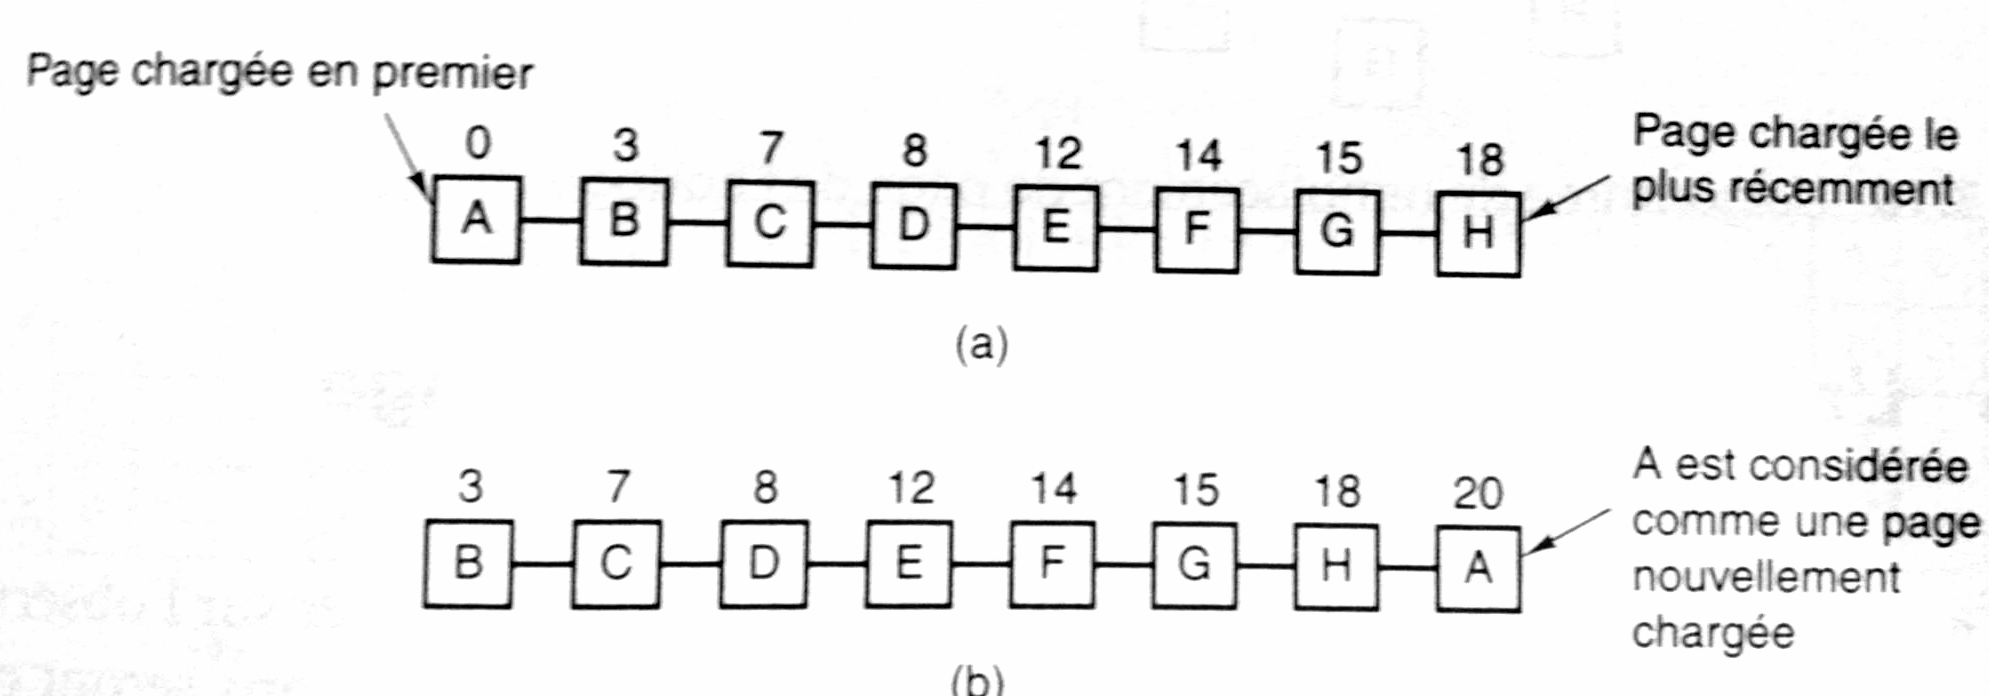
\includegraphics[scale=0.2]{images/sequencedepage.png}
	\caption{\label{Sequence de pages} Séquence de pages}
\end{figure}
\color{reponse}
\begin{itemize}
	\item La première page contenant un bit 0 sera choisie, dans ce cas \textit{D}.
\end{itemize}
\color{black}



\paragraph{Question 6} (Mémoire). Une page peut-elle se trouver dans deux ensembles de travail en même temps ? Expliquez.
\color{reponse}
\begin{itemize}
	\item Si l'on peut partager les pages, oui. Par exemple, si deux utilisateurs d'un système en temps partagé exécutent le même éditeur au même moment et que le texte du programme est partagé au lieu d'être copié, certaines de ces pages peuvent se trouver simultanément dans l'espace de travail de chaque utilisateur.
\end{itemize}
\color{black}